{\chapter{Analyse}}
\label{sec:analyse}
Zusätzlich zu den maschinellen Lernkomponenten stellt Unity auch Demonstrationsumgebungen bereit, in denen verschiedene Lösungen für gängige Verstärkungslernprobleme implementiert sind. In der Walker-Demo wird ein physisch simulierter Charakter darauf trainiert, zu einem Zielwürfel zu laufen. Diese Demo-Umgebung implementiert bereits einige Grundlagen für die Steuerung eines physisch simulierten Charakters. Aus diesem Grund wird in dieser Arbeit die Walker-Demo als Basis für die Entwicklung genutzt. In diesem Kapitel wird daher die Walker-Demo analysiert, um in den folgenden Kapiteln darauf aufzubauen.

\section{Szenenaufbau}
Die Szene besteht aus einem quadratischen Spielfeld mit Boden und Wänden die der Charakter nicht verlassen kann (siehe Abbildung \ref{fig:walker_aufbau}). Des Weiteren beinhaltet die Umgebung noch den Läufer und das Ziel zu welchem der Läufer lernt zu laufen.
\begin{figure}[H]
  \centering  
  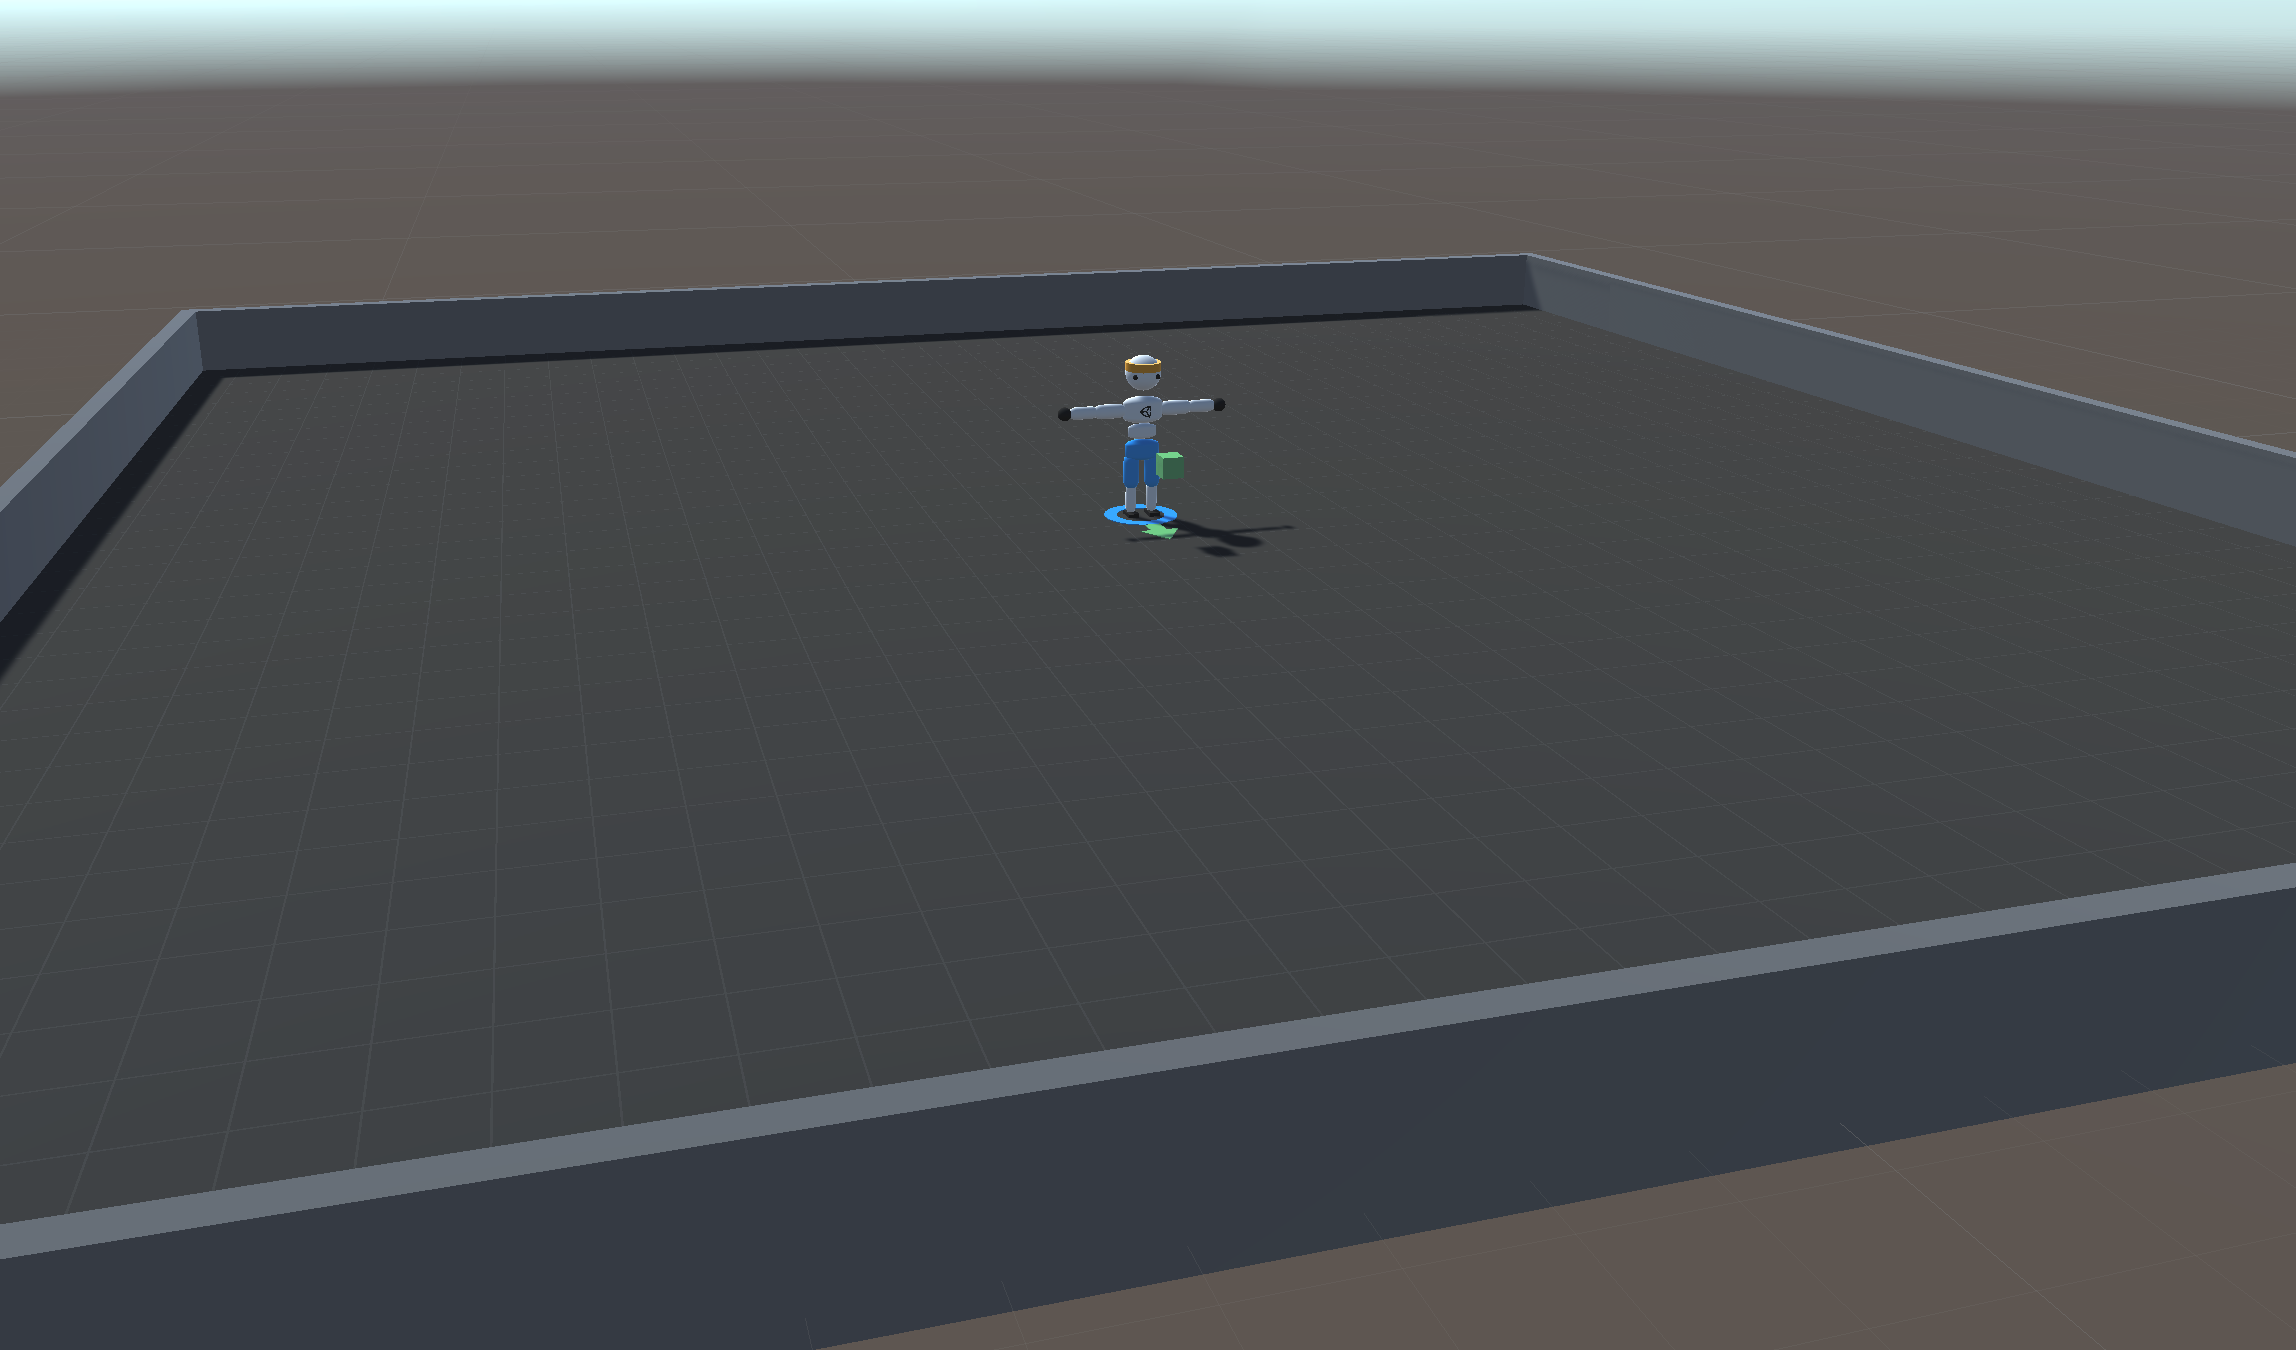
\includegraphics[scale=0.35]{img/walker_aufbau.png}
  \caption{Walker-Demo Szenenaufbau}
  \label{fig:walker_aufbau}
\end{figure}

\section{Läufer}
Der Körper des Läufers besteht aus 11 Kapseln, drei Kugeln und 2 Quadern, jeder dieser Formen hat eine Festkörper und eine Kollisions Physikkomponente. Zwischen den Körperteilen werden die Gelenke als Kugelgelenke simuliert. Die genaue Physikkonfiguration der Körperteile werden veranschaulicht in Tabelle \ref{table:walker_körperteile}

\begin{table}[H]
  \centering
  {\rowcolors{1}{gray!10}{white}
  \begin{tabular}{ |p{3cm}|p{3cm}|p{2cm}|p{4cm}|p{2cm}| }
  \hline
  \textbf{Körpertei}l& \textbf{Verbundenes Körperteil} & \textbf{Gewicht} & \textbf{Winkellimits} & \textbf{Form} \\
  \hline
  Hüfte & - & 15kg & - & Kapsel \\
  \hline
  Wirbelsäule & Hüfte & 10kg & x(-20,20) y(-20,20) z(-15,15) & Kapsel \\
  \hline
  Oberkörper & Wirbelsäule & 8kg & x(-20,20) y(-20,20) z(-15,15) & Kapsel \\
  \hline
  Kopf & Oberkörper & 6kg & x(-30,10) y(-20,20) & Kugel \\
  \hline
  Oberarm LR & Oberkörper & je 4kg & x(-60,120) y(-100,100) & Kapsel \\
  \hline
  Unterarm LR & Oberarm & je 3kg & x(0,160) & Kapsel \\
  \hline
  Hand LR & Unterarm & je 2kg & - & Kugel \\
  \hline
  Oberschenkel LR & Hüfte & je 14kg& x(-90,60) y(-40,40) & Kapsel \\
  \hline
  Unterschenkel LR & Oberschenkel & je 7kg &  x(0,120) & Kapsel \\
  \hline
  Fuß LR & Unterschenkel & je 5kg & x(-20,20 y(-20,20) z(-20,20) & Quader \\
  \hline
  \end{tabular}}
  \caption{Walker Agent Körperteile}
  \label{table:walker_körperteile}
\end{table}

Gesteuert wird der Läufer über die Gelenk Motor Steuerung (Joint Drive Controller). Das Walker Agent Skript registriert die Körperteile bei der Initialisierung in der Gelenk Motor Steuerung. Anschließend können über die Gelenk Motor Steuerung die Zielrotationen sowie die Maximale Kraft des Gelenks festgelegt werden, und somit der Läufer gesteuert werden. Die Gelenk Motor Einstellungen (Joint Drive Settings) siehe Abbildung \ref{fig:agent_konfiguration} \hl{bestimmen die Stärke mit welcher die Gelenke in die Zielstellung bewegt werden.}
\begin{itemize}
  \item Max Joint Spring: Bestimmt den Drehmoment mit welchem das Gelenk in die Zielposition rotiert wird.
  \item Joint Dampen: Verringert den Drehmoment proportional zur Differenz zwischen aktueller Geschwindigkeit und der Zielgeschwindigkeit. Verringert Schwingungen.
  \item Max Joint Force Limit: Gibt die maximale Kraft des Gelenks an (verhindert zu schnelle Bewegung bei großer Abweichung).
\end{itemize}
\begin{figure}[H]
  \centering  
  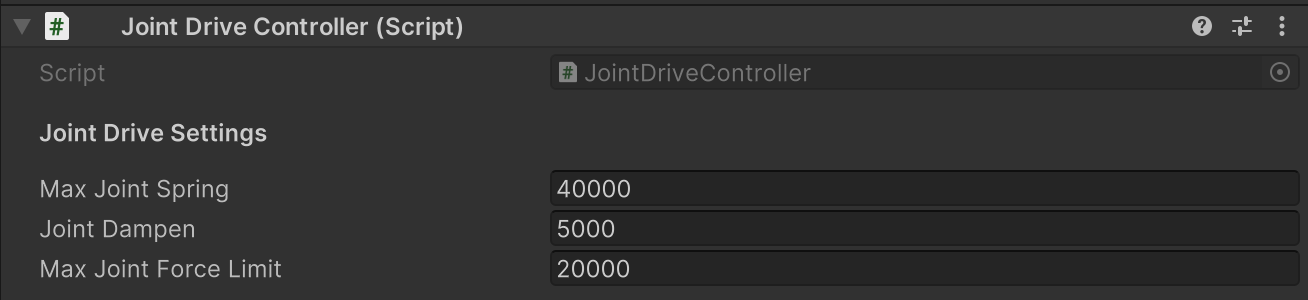
\includegraphics[scale=0.5]{img/gelenk_motor_steuerung.png}
  \caption{Gelenk Motor Steuerung}
  \label{fig:gelenk_motor_steuerung}
\end{figure}


\section{Agent}
Das Walker Agent Skript, definiert den Läufer als Agent für das maschinelle Lernen. Abbildung \ref{fig:agent_konfiguration} zeigt die Agentenkomponente im Inspektor. Um die Komponente zu nutzen müssen hier die Körperteile des Walkers referenziert werden. Zusätzlich kann eine Zielgeschwindigkeit festgelegt werden und ob die Geschwindigkeit variieren soll während dem Training. Als letztes muss auch das Zielobjekt referenziert werden.
\begin{figure}[H]
  \centering  
  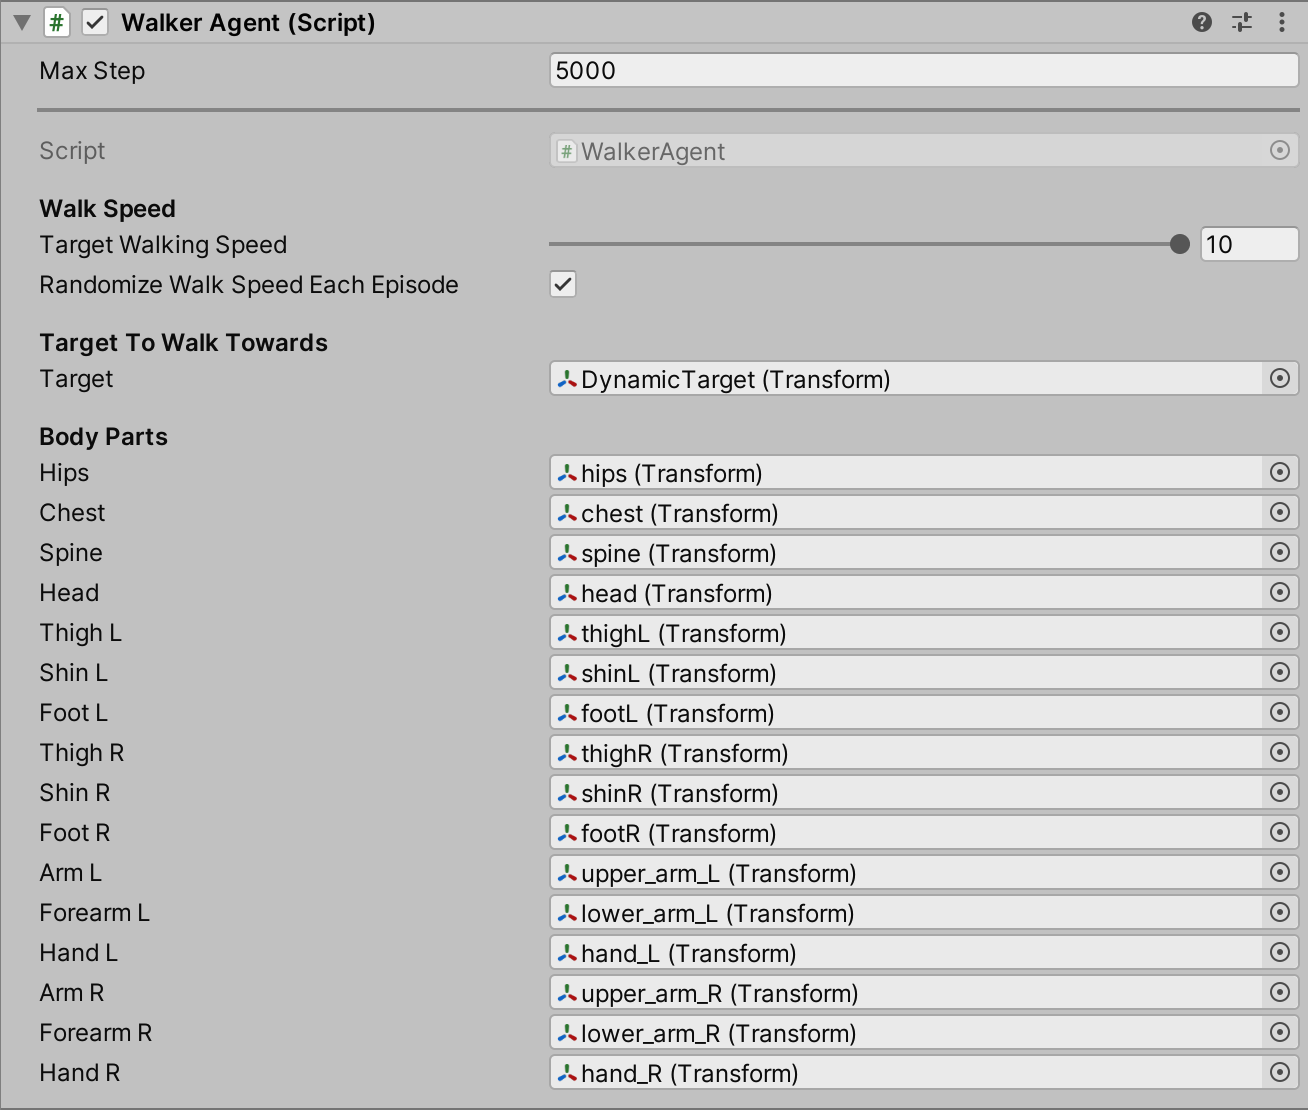
\includegraphics[scale=0.5]{img/agent_konfiguration.png}
  \caption{Agent Konfiguration}
  \label{fig:agent_konfiguration}
\end{figure}

Die Beobachtung des Agenten wird in Tabelle \ref{table:walker_beobachtung} dargestellt.\\
\begin{table}[H]
  \centering
  {\rowcolors{1}{gray!10}{white}
  \begin{tabular}{ |p{1cm}|p{9cm}|p{5cm}|}
  \hline
  \textbf{ID} & \textbf{Beobachtung} & \textbf{Anmerkung}  \\
  \hline
  \rowids & Abweichung Durchschnittsgeschwindigkeit von Zielgeschwindigkeit &  \\
  \hline
  \rowids & Durchschnittsgeschwindigkeit &  \\
  \hline
  \rowids & Zielgeschwindigkeit & \\
  \hline
  \rowids & Abweichung Hüftrotation von Zielrotation & \\
  \hline
  \rowids & Abweichung Kopfrotation von Zielrotation & \\
  \hline
  \rowids & Zielposition & \\
  \hline
  \rowids & Körperteil Beobachtungen & Beobachtung aus Tabelle \ref{table:walker_beobachtung_körperteil} für jedes Körperteil \\
  \hline
  \end{tabular}}
  \caption{Walker Agent Beobachtung}
  \label{table:walker_beobachtung}
\end{table}
\rowidsclear

Für jedes Körperteil wird die folgende Beobachtung dem Zustand angefügt.\\
\begin{table}[H]
  \centering
  {\rowcolors{1}{gray!10}{white}
  \begin{tabular}{ |p{1cm}|p{9cm}|p{5cm}|}
  \hline
  \textbf{ID} & \textbf{Beobachtung} & \textbf{Anmerkung}  \\
  \hline
  \rowids & Bodenkontakt & \\
  \hline
  \rowids & Geschwindigkeit & \\
  \hline
  \rowids & Rotationsgeschwindigkeit & \\
  \hline
  \rowids & Position relativ zur Hüfte & \\
  \hline
  \rowids & LokaleRotation & Fehlt für Hüfte und Hände \\
  \hline
  \rowids & Gelenkstärke & Fehlt für Hüfte und Hände \\
  \hline
  \end{tabular}}
  \caption{Walker Agent Körperteil Beobachtung}
  \label{table:walker_beobachtung_körperteil}
\end{table}
\rowidsclear

Das Format einer Aktion besteht aus den in Tabelle \ref{table:walker_aktion} aufgeführten Feldern für jedes Körperteil des Läufers, ausgenommen der Hüfte und Hände.\\
\begin{table}[H]
  \centering
  {\rowcolors{1}{gray!10}{white}
  \begin{tabular}{ |p{1cm}|p{9cm}|p{5cm}|}
  \hline
  \textbf{ID} & \textbf{Beobachtung} & \textbf{Anmerkung}  \\
  \hline
  \rowids & Rotationswinkel X & Nur wenn Körperteil X Rotation beweglich ist\\
  \hline
  \rowids & Rotationswinkel Y & Nur wenn Körperteil Y Rotation beweglich ist\\
  \hline
  \rowids & Rotationswinkel Z & Nur wenn Körperteil Z Rotation beweglich ist\\
  \hline
  \rowids & Gelenkstärke & \\
  \hline
  \end{tabular}}
  \caption{Walker Agent Aktion}
  \label{table:walker_aktion}
\end{table}
\rowidsclear

Die Belohnungsfunktion enthält zwei Komponenten. Zum einen wird die Differenz der Bewegung in Zielrichtung zwischen momentaner Bewegung und Zielbewegung durch die Funktion $R_V$ bewertet. Zum Anderen wird die Abweichung zwischen momentaner Blickrichtung und der Zielrichtung in $R_L$ berechnet. Die Belohnung ergibt sich am ende durch die Multiplikation beider Teilterme. Die Verwendung der Multiplikation hat zur Folge das die Belohnung gleichermaßen von beiden Teiltermen abhängig ist und es somit notwendig ist, beide Teile gleichzeitig zu optimieren.\\
\begin{figure}[H]
  \centering  
  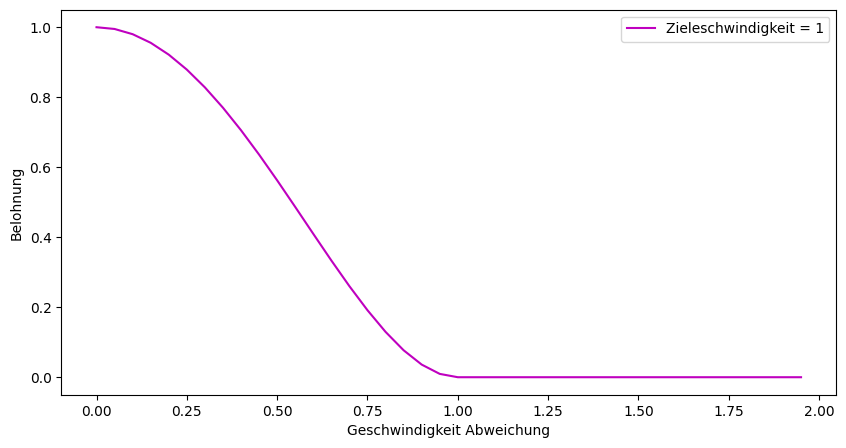
\includegraphics[scale=0.5]{img/match_velocity_demo_vel1.png}
  \caption{Walker Demo Match Velocity Belohnungsfunktion}
  \label{fig:match_velocity_demo_vel1}
\end{figure}
$V_\delta=Clip(|\vec{Geschwindigkeit} - \vec{Zielgeschwindigkeit}|, 0, |\vec{Zielgeschwindigkeit}|)$ \\
$R_V=(1 - (V_\delta / |\vec{Zielgeschwindigkeit}|)^2)^2$ \\
\begin{figure}[H]
  \centering  
  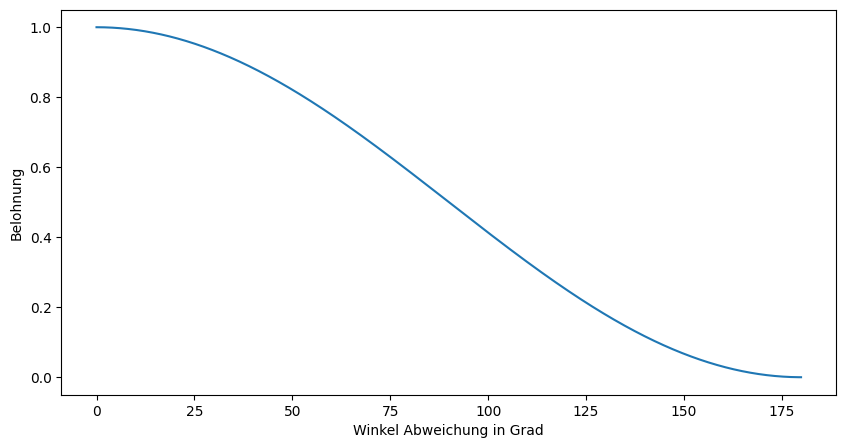
\includegraphics[scale=0.5]{img/look_at_target_demo.png}
  \caption{Walker Demo Look At Target Belohnungsfunktion}
  \label{fig:look_at_target_demo}
\end{figure}
$R_L=(\vec{Zielrichtung} \cdot \vec{Blickrichtung})+ 1) \cdot 0.5$ \\
$R=R_V \cdot R_L$

Initialisierung bzw Episodereset erklären
Orientation Object erklären
Zielsetzung erklären
Rewardfrequenz erwähnen